\documentclass[border=10pt]{standalone}
\usepackage{tikz}
\usetikzlibrary{arrows,positioning}
\begin{document}
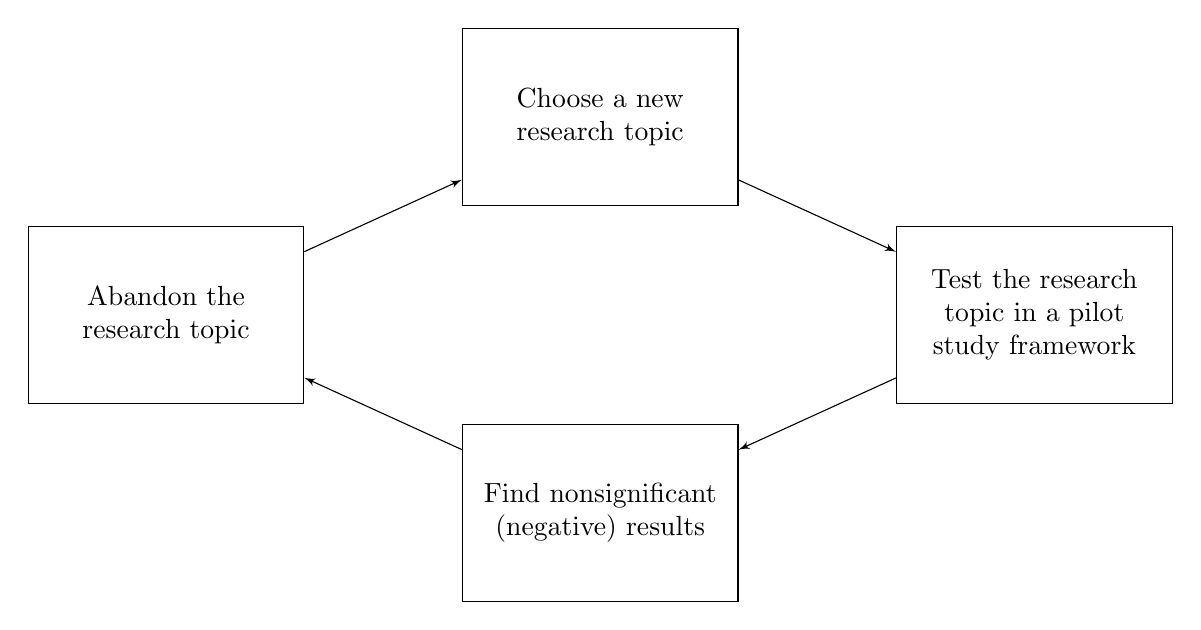
\begin{tikzpicture}[>=latex']
  \tikzset{block/.style= {draw, rectangle, align=center,minimum
      width=3.5cm,minimum height=2.25cm}}
  \node[block] (start) {Choose a new\\research topic};
  \node[block, below right =0.25cm and 2cm of start] (next) {Test the research\\topic in a
    pilot\\study framework};
  \node[block, below left =0.25cm and 2cm of next] (next2) {Find nonsignificant\\(negative)
    results};
  \node[block, below left =0.25cm and 2cm of start] (next3) {Abandon the\\research topic};
  
  \path[draw, ->] (start) edge (next);
  \path[draw, ->] (next) edge (next2);
  \path[draw, ->] (next2) edge (next3);
  \path[draw, ->] (next3) edge (start);
\end{tikzpicture}
\end{document}

%%% Local Variables: 
%%% mode: latex
%%% TeX-master: t
%%% End: 
